\section{Durchführung}
\label{sec:Durchführung}

In Abbildung 3 ist der Aufbau skizziert. Ein Laser mit Wellenlänge $\lambda = 635 \si{\nano\meter}$ fällt auf einen Spalt. In einem Meter Entfernung befindet sich ein Detektor, bestehend aus einer Photodiode. Der Detektor kann mittels eines Messverschiebereiters verschoben werden.
An einem mit dem Detektor verbundenen Amperemeter wird die Stromstärke abgelesen.
\begin{figure}[H]
  \centering
  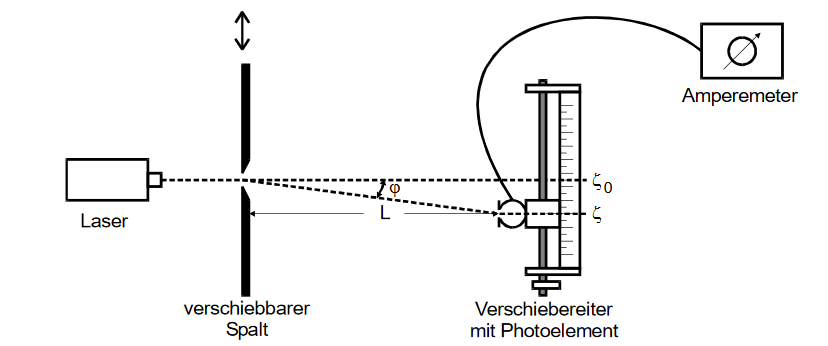
\includegraphics[height=6cm]{aufbau.PNG}
  \caption{Versuchsaufbau zur Bestimmung der Beugungsfiguren.\cite{kent}.}
\end{figure}

\noindent Zuerst muss der Dunkelstrom des Photoelements bestimmt werden, also der beim ausgeschalteten Laser gemessene Strom.
Es werden zwei Einzelspalte mit unterschiedlicher Breite benutzt. Es muss darauf geachtet werden, dass der Detektor gerade ist um die Beugungsbilder richtig zu vermessen.
Zur Justierung wird das Hauptmaximum mit dem Messverschiebereiter in die Mitte des Detektorspalts geschoben. Die Nebenmaxima sollen etwa die gleiche Intensität haben.

\noindent Um die Beugungsfigur auszumessen, wird die Intensität in Abhängigkeit von der Detektorstellung gemessen. Dazu wird der Detektor immer soweit verschoben, bis die Maxima und Minima auf dem Amperemeter angezeigt werden. Es muss darauf geachtet werden, dass genug Werte im Bereich der Nebenmaxima und Nebenminima aufgenommen werden, damit ein gutes Beugungsbild geplottet werden kann.
50 Intensitäten und zugehörige Detektorstellungen werden notiert. 
Sind die Messungen abgeschlossen, wird gleiches mit einem Doppelspalt durchgeführt.
